% Chapter Template
\chapter{Original Data Analysis} % Main chapter title

\label{Chapter3} % Change X to a consecutive number; for referencing this chapter elsewhere, use \ref{ChapterX}

%----------------------------------------------------------------------------------------
%	SECTION 1
%----------------------------------------------------------------------------------------

\section{Full Model Estimation}

 As we have mentioned, we did the data pre-processing before we begin our data analysis (model fitting). We analyzed this set of data according to the most
 fundamental steps of regression analysis. This is the analysis of the full model.
Our Full model's regression formula is :

\begin{align*}
  \centering
PM2.5 = \beta_0 + \beta_1\text{timestamp} + \beta_2\text{season} + \beta_3\text{Iws} + \beta_4\text{Is} + \beta_5\text{Ir} + \beta_6\beta\text{DEWP} + \beta_7\text{TEMP} + \beta_8\text{PRESS} + \beta_9\text{cbwd_data}
\end{align*}


The model's summary are given below:
\\
\\
\begin{tabular}{|c|c|c|c|c|}
\hline       beta   &    Estimate & Std. Error &t value &Pr(>|t|)    \\
\hline (Intercept)  & 2.344e+03  &5.414e+02 &  4.329 &1.71e-05 *** \\
\hline timestamp    & -4.383e-04 & 1.178e-02&  -0.037& 0.970337    \\
\hline seasonSpring & 2.530e+01  &8.012e+00  & 3.158 &0.001654 **  \\
\hline easonSummer  & -3.362e+01 & 8.985e+00 &-3.742 &0.000197 *** \\
\hline seasonWinter & 2.408e+01  &9.346e+00  & 2.576 &0.010193 *   \\
\hline Iws          & -1.657e-01 & 6.586e-02 & -2.516& 0.012075 *   \\
\hline Is           & -1.544e+01 & 6.509e+00 & -2.372& 0.017953 *   \\
\hline Ir           & -1.493e+01 & 2.967e+00 & -5.032 &6.13e-07 *** \\
\hline DEWP         & 7.567e+00  &5.021e-01  &15.070  &< 2e-16 *** \\
\hline TEMP         & -1.053e+01 & 7.359e-01 &-14.310 & < 2e-16 *** \\
\hline PRES         & -2.056e+00 & 5.292e-01 & -3.885 &0.000112 *** \\
\hline cbwd\_dataNE  & -6.115e+01 & 1.226e+01 & -4.988 &7.66e-07 *** \\
\hline cbwd\_dataNW  & -2.927e+01 & 7.431e+00 & -3.939 &9.00e-05 *** \\
\hline cbwd\_dataSE  & -1.883e+01 & 6.793e+00 & -2.772 &0.005710 **  \\
\hline
\end{tabular}
\\
\\

Which is in the form of: $y = \beta_1 x_1 + \dots + \beta_9 x_9 \label{eq: Full Model}$

Initally, to come up with the full model, we decided to first plot correlation plots for all regressors that we believed taht may have a constant variance: See \refeq{fig:Correlation of the full model}

\begin{figure}[H]
    \centering
  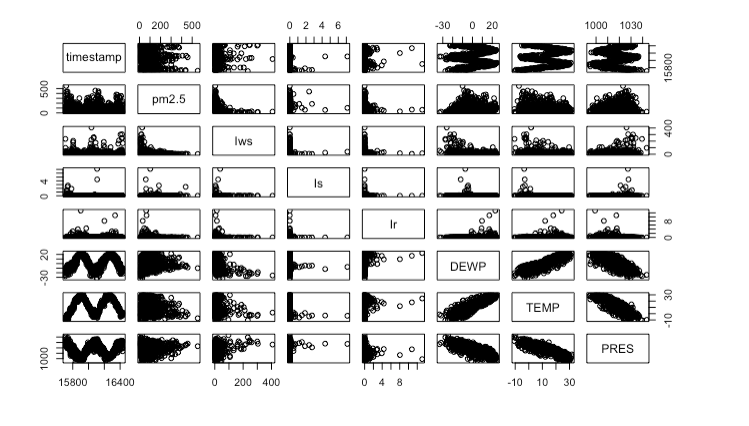
\includegraphics[width=1.0\textwidth]{Figures/correlationfull.png}
  \caption[Figures/correlation\_full.png]{Correlation of the full model}
  \label{fig:Correlation of the full model}
\end{figure}

From \ref{fig:Correlation of the full model}, we noticed that the correlation between PM2.5 and cumulated hour of wind speed(Iws), cumulative hours of snow(Is), and cumulative hours of rain(Ir) are all strong and their correlation density curve  seem like all right skewed. We can use the 'Residuals vs Fitted' plot and the 'Normal Q-Q' plot of residual to check whether our deduction.


The $`lm`$ function can also plots out the 'Residuals vs Fitted' plot, 'Normal Q-Q'plot, 'Scale-Location' and 'Residuals vs Leverage' plot: See \refeq{fig:Testing Plots of Full Model}

\begin{figure}[H]
  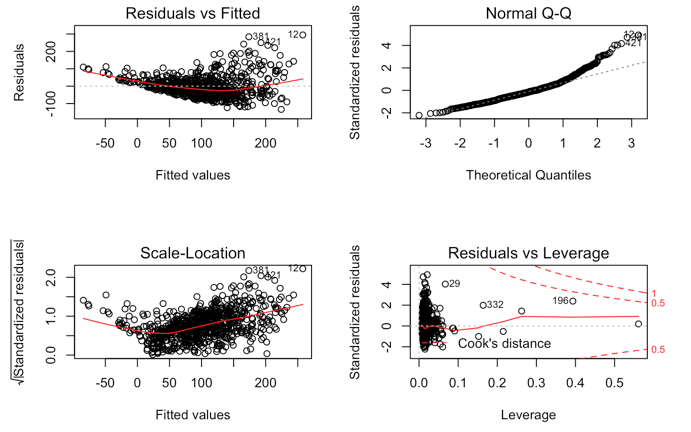
\includegraphics[width=1.0\textwidth]{Figures/lm_full.png}
  \caption[Figures/lm\_full.png]{Four testing plots}
  \label{fig:Testing Plots of Full Model}
\end{figure}

We also use lm and vif function to check the vif value of each variables. The result shows that all the variables’ vif value are not way larger than 10. The largest one is approximately $13.4$, which means the variables don’t have a high multicolliearity and the model has no compressibility. We can’t do the ridge regression and also the lasso regression to this model.

\section{Model with Natural Logrithm}
It can be seen that the residual of the  full model \ref{eq: Full Model} is nonlinear. Usually, we need to do the \textbf{ncv test} to check want kinds of transformation should we do, however, according the reference book, we can do the Natural Logarithm transforamtion to the dependent variable when the residual plot is right skewed the\citep{montgomery2012introduction}.  Then we take the natural logarithm of the dependent variable, thus obtaining a new regression model: Full Model with Natural Logarithm Transformation, by comparing the residual graphs of the two models, we can clearly see that the residual of the model after natural logarithm transformation is linear, but we can see the residuals plot as the double-bow model\citep{montgomery2012introduction}, which represents the model at this time. The variance of the residuals is not the same, and it does not satisfy the characteristics of the regression model of homoscedasticity.

Here is the formula of the model after the Natural Logarithm transformation:

\begin{align*}
  \centering
  log(PM2.5) = \beta_0 + \beta_1\text{timestamp} + \beta_2\text{season} + \beta_3\text{Iws} + \beta_4\text{Is} + \beta_5\text{Ir} + \beta_6\beta\text{DEWP} + \beta_7\text{TEMP} + \beta_8\text{PRESS} + \beta_9\text{cbwd_data}
\end{align*}
Which is in form of :
$log(y) = \beta_1 x_1 + \dots + \beta_9 x_9 \label{eq: Full Model with Natural Logarithm}$

\begin{figure}[H]
  \centering
  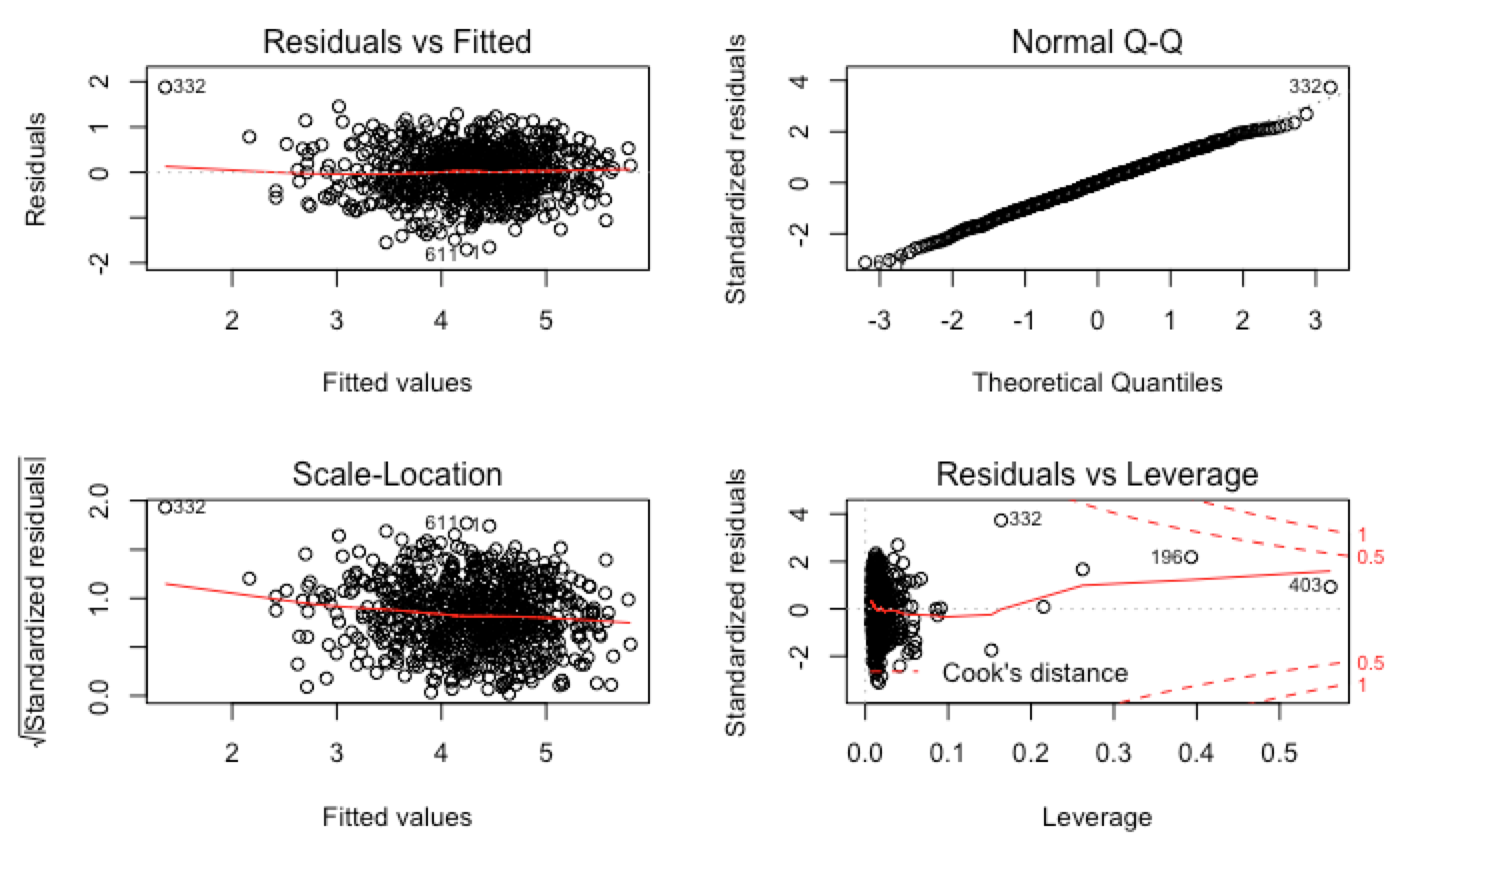
\includegraphics[width=1.0\textwidth]{Figures/lm_full_nl.png}
  \caption[Figures/lm\_full\_nl.png]{Full Model with Natural Logarithm test plot}
  \label{fig:Full Model with Natural Logarithm test plot}
\end{figure}

\section{Interaction Model}
According to the \ref{fig:Correlation of the full model}, there are some correlations between some of the independent variables and dependent variable,
It can be seen that although the residual at this time is in accordance with the normal distribution, it can be seen from the residual map that the variance of the residuals is not the same. We suspect that there are interactions between different variables, so we have newly created a model to try to improve the $R^2$ of the model, and then filter the model through stepwise method.

The Interaction Model is:
\\
\\
\begin{align*}
  \centering
  log(PM2.5) = ()\beta_0 + \beta_1\text{timestamp} + \beta_2\text{season} + \beta_3\text{Iws} + \beta_4\text{Is} + \beta_5\text{Ir} + \beta_6\beta\text{DEWP} + \beta_7\text{TEMP} + \beta_8\text{PRESS} + \beta_9\text{cbwd_data})^2
\end{align*}
\\
\\
\begin{figure}[H]
  \centering
  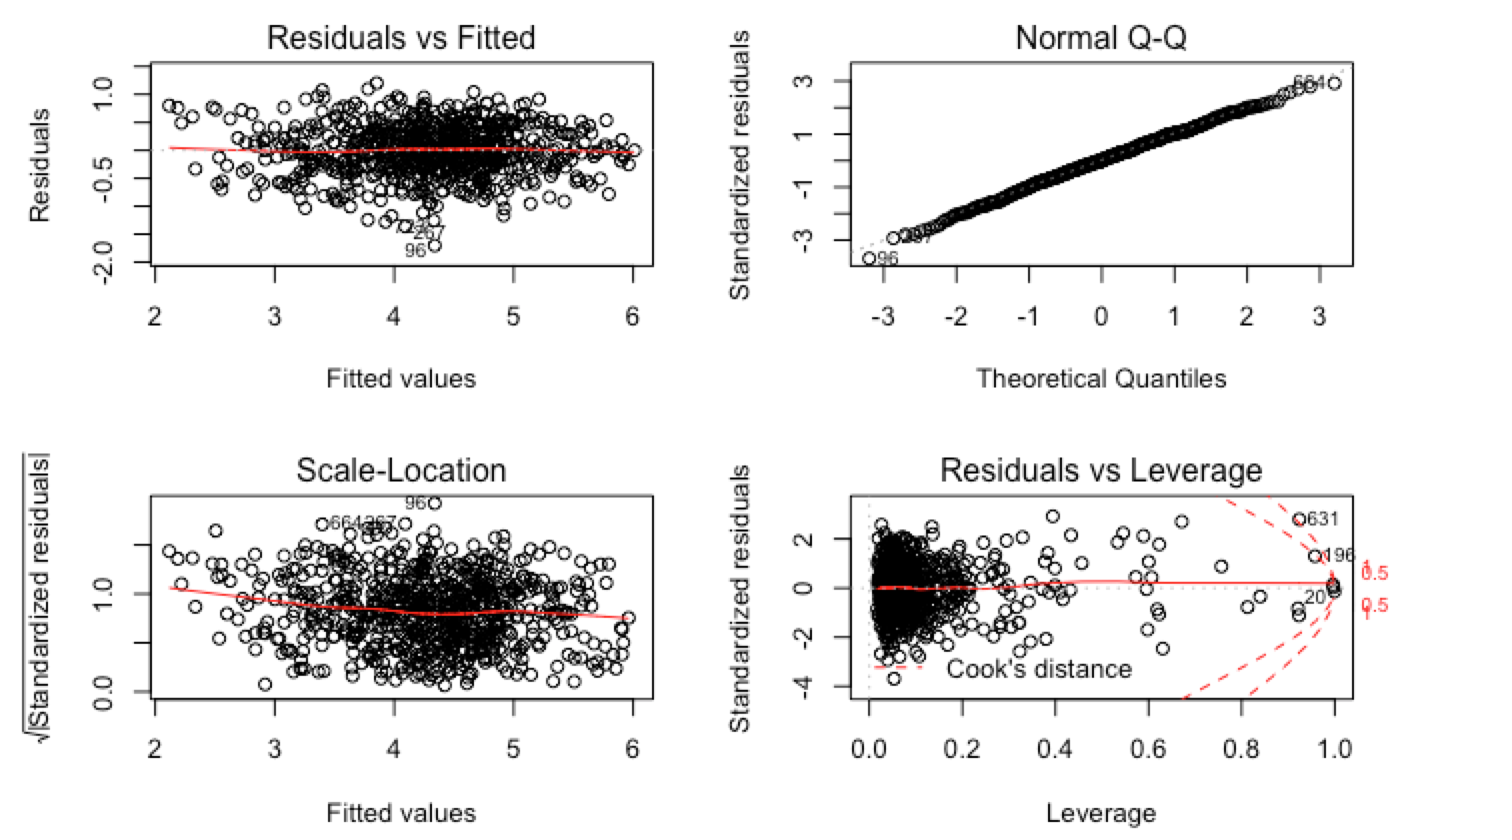
\includegraphics[width=1.0\textwidth]{Figures/lm_full_in.png}
  \caption[Figures/lm\_full\_in.png]{Natural Logarithm Model with Interaction}
  \label{fig:Natural Logarithm Model with Interaction}
\end{figure}

As we can see in the \ref{fig:Natural Logarithm Model with Interaction}, the  variance is more dispersed, the homoscedasticity is better, and R square($R^2 = 0.7086$) is higher.

\section{Stepwise Method}

In Statistics, we usually use Stepwise to choose the variables, choose the predictive varaibles by the R's built-in automatic procedure.
At the beginning, the AIC = $-1001.82$ and at the last step, the AIC = $-1035,45$, and the
model selected by AIC is:

\begin{align*}
\centering
log(pm2.5)  = timestamp + season + Iws + Is + Ir + DEWP + TEMP +
    PRES + cbwd_data + timestamp:season + timestamp:Is + timestamp:cbwd_data +
    season:Iws + season:DEWP + season:TEMP + season:PRES + season:cbwd_data +
    Iws:Ir + Iws:DEWP + Iws:TEMP + Iws:PRES + Iws:cbwd_data +
    Is:TEMP + Is:PRES + Ir:DEWP + Ir:TEMP + Ir:PRES + DEWP:PRES +
    TEMP:cbwd_data + PRES:cbwd_data + intercept
\end{align*}
The R square now is $0.6995$ and the test plots is much better than before, see \ref{fig:Stepwise Model}
\begin{figure}[H]
  \centering
  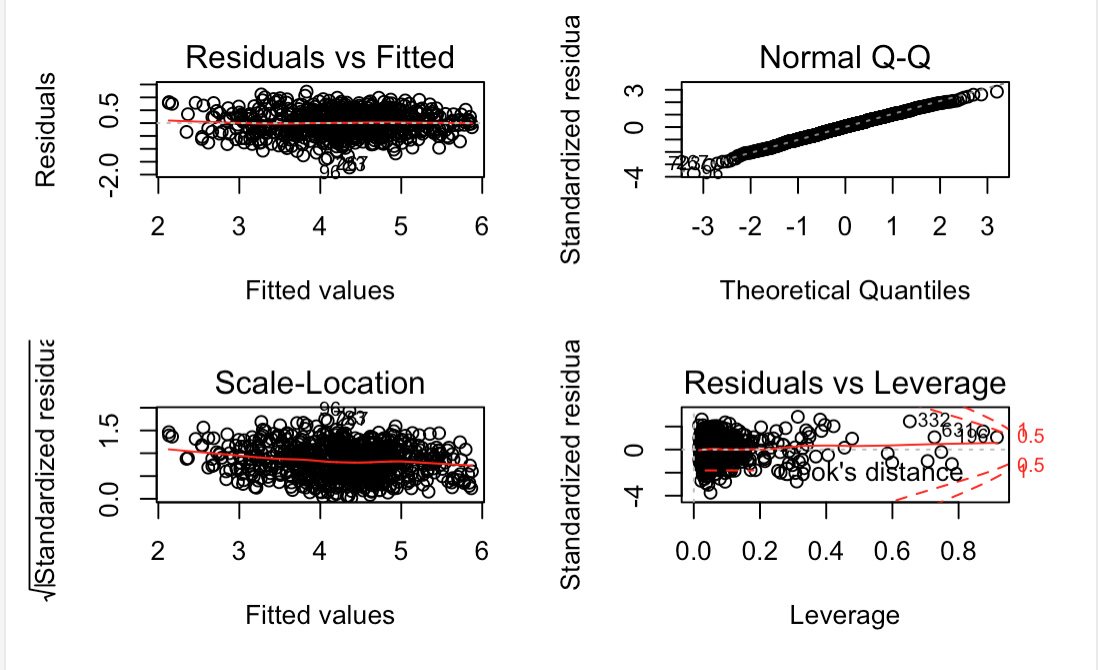
\includegraphics[width=1.0\textwidth]{Figures/lm_full_in_step.png}
  \caption[Figures/lm\_full\_in\_step.png]{Stepwise Model}
  \label{fig:Stepwise Model}
\end{figure}
Although it seem like a good model, in some ways, we thought it was not a fitted model we want.
After checking the original variables again, we found that the Cumulated hours of snow , Dew Point and Temperature thereT all have strong correlation with time. Then, we came up a new idea, we have to separate the time as a more smaller segments in terms of season as unit. Usually, smog is more likely to affect humans in the spring and winter seasons. This can be reflected in the previous model. The correlation between spring and winter and pm2.5 is much larger than that in summer and autumn.
Then, we chose Spring + Winter as the time nodes and continue our model estimation.
